\chapter{Resultados e discussão}

\thispagestyle{plain}
\section{Estimativa do parâmetro $\rho$ da fórmula da REN}


Com o $\rho_{proposto}$, calculado através da fórmula \ref{eq:rhoproposed}, arredondado a uma casa decimal, podemos verificar no histograma, apresentado na figura \ref{fig:histograma_parametro_p}, uma diferença considerável entre as contagens de ambos os conjuntos de valores $\rho$ apresentados.\par


% \begin{figure}[H]
%     \centering
%     \includegraphics[width=0.7\textwidth]{plots/histograma_parâmetro_ρ.png}
%     \caption{Histograma $\rho$}
%     \label{fig:histograma_parametro_p}
%   \end{figure}


% \begin{figure}[H]
%     \centering
%     \includegraphics[width=0.65\textwidth]{plots/valor_do_parametro_ρ_(hora).png}
%     \caption{Valor do paramêtro $\rho$ (hora)}
%     \label{fig:valor_do_parametro_ρ_hora}
%   \end{figure}

\begin{figure}[H]
    \centering
    % First figure in a minipage
    \begin{minipage}[b]{0.49\textwidth}
        \centering
        \includegraphics[width=\textwidth]{plots/histograma_parâmetro_ρ.png}
        \caption{Histograma $\rho$}
        \label{fig:histograma_parametro_p}
    \end{minipage}
    % Second figure in a minipage
    \begin{minipage}[b]{0.49\textwidth}
        \centering
        \includegraphics[width=\textwidth]{plots/valor_do_parâmetro_ρ_(hora).png}
        \caption{Valor do parâmetro $\rho$ (hora)}
        \label{fig:valor_do_parametro_ρ_hora}
    \end{minipage}
\end{figure}

Como podemos ver na figura \ref{fig:valor_do_parametro_ρ_hora}, acima apresentada, o $\rho_{proposto}$ apresenta um grande variabilidade em todas as horas, embora de notar que em todas tem um maior peso perto da mediana. O $\rho$ de comparação embora sempre dentro da distribuição note-se que cai quase sempre em zonas com pouco peso nestes dados históricos.\par
Calculamos $\rho$ possíveis para proposta final usando as seguintes aproximações: média, mediana, \gls{mp-consumo} e \gls{mp-BS}.\par

As distribuições por hora são as apresentadas na seguinte figura:

\begin{figure}[H]
    \centering
    \includegraphics[height=0.42\textwidth]{plots/comparação_de_ρ_propostos_por_hora.png}
    \caption{Comparação $\rho$ por hora}
    \label{fig:comparação_de_ρ_propostos_por_hora}
\end{figure}

Todas seguem um percurso semelhante ao longo do dia, o qual também pode ser extrapolado para Carneiro2016. A média e mediana destacam-se seguindo muito parecidas, enquanto que as ponderadas também parecidas entre elas são bastante mais discretas.\par
Para a escolha da aproximação deste parâmetro à Hora, estudou-se o erro entre a Banda Reserva calculada através das aproximações feitas e a Banda Reserva disponível nos dados.\par


\begin{figure}[H]
    \centering
    \includegraphics[width=0.7\textwidth]{plots/comparação_das_métricas_de_erro.png}
    \caption{Comparaçao dos erros por $\rho$}
    \label{fig:comparação_das_métricas_de_erro}
\end{figure}


\begin{table}[H]
    \centering
    \caption{Erros de Banda de Reserva por método de normalização $\rho$}    
    \resizebox{0.65\linewidth}{!}{\begin{tabular}{lrrrr}
\toprule
 & MAE (MW) & RMSE (MW) & MedianAE (MW) & MAPE (\%)\\
Normalização &  &  &  &  \\
\midrule
Carneiro2016 & 53.07 & 66.54 & 44.53 & 18.70 \\
média & 30.94 & 39.19 & 25.38 & 11.58 \\
mediana & 30.85 & 39.20 & 25.17 & 11.51 \\
média ponderada banda & 32.15 & 40.61 & 26.45 & 12.19 \\
média ponderada consumo & 31.54 & 39.91 & 26.20 & 11.73 \\
\bottomrule
\end{tabular}
}
    \label{fig:tabela_estudo_1_medias}
    \end{table}


A normalização com erros mais baixos é a média. Com um erro médio (de todo o histórico) para o consumo real de 8.8\% o que comparando com o \textit{benchmark} de 29.36\% é uma melhoria  bastante considerável. Comparando as bandas calculadas a uma média em cada hora:\par

\begin{figure}[H]
    \centering
    \includegraphics[width=0.75\textwidth]{plots/média_historica_de_banda_de_reserva.png}
    \caption{Média historica de Banda de Reserva}
\end{figure}

Podemos ver que em termos de média horária, a Banda de Reserva calculada através do $\rho_{proposto}$ apresenta quase uma sobreposição por inteiro ao valor médio real.\par

Retiramos as médias dos erros percentuais e podemos observar: \\

\begin{figure}[H]
    \centering
    \includegraphics[width=0.75\textwidth]{plots/erro_médio_por_hora_banda_de_reserva.png}
    \caption{Erro médio por hora Banda de Reserva}
\end{figure}

Em termos de média diária o erro pelo método proposto está bem abaixo da margem de erro do 5\% na banda, em todas as horas. E na outra tese apenas 10\% cai dentro dessa margem de erro.\par

Como tal o $\rho_{proposto}$ a partir do estudo dos dados  históricos é: \

\begin{table}[H] \centering \caption{Valores de $\rho$ propostos} \begin{tabular}{rr}
\toprule
Hora & $\rho$ \\
\midrule
1 & 1.621694 \\
2 & 1.576623 \\
3 & 1.486929 \\
4 & 1.364176 \\
5 & 1.313958 \\
6 & 1.318832 \\
7 & 1.504499 \\
8 & 1.612361 \\
9 & 1.638188 \\
10 & 1.613728 \\
11 & 1.601277 \\
12 & 1.485861 \\
13 & 1.451995 \\
14 & 1.457233 \\
15 & 1.440454 \\
16 & 1.421988 \\
17 & 1.424636 \\
18 & 1.420682 \\
19 & 1.553086 \\
20 & 1.588201 \\
21 & 1.480219 \\
22 & 1.478815 \\
23 & 1.474412 \\
24 & 1.635658 \\
\bottomrule
\end{tabular}
 \end{table}


% \begin{table}[H]
%     \caption{Valores de $\rho$ propostos}    
%     \resizebox{\linewidth}{!}{\begin{tabular}{rr}
\toprule
Hora & $\rho$ \\
\midrule
1 & 1.621694 \\
2 & 1.576623 \\
3 & 1.486929 \\
4 & 1.364176 \\
5 & 1.313958 \\
6 & 1.318832 \\
7 & 1.504499 \\
8 & 1.612361 \\
9 & 1.638188 \\
10 & 1.613728 \\
11 & 1.601277 \\
12 & 1.485861 \\
13 & 1.451995 \\
14 & 1.457233 \\
15 & 1.440454 \\
16 & 1.421988 \\
17 & 1.424636 \\
18 & 1.420682 \\
19 & 1.553086 \\
20 & 1.588201 \\
21 & 1.480219 \\
22 & 1.478815 \\
23 & 1.474412 \\
24 & 1.635658 \\
\bottomrule
\end{tabular}
}
%     \end{table}

% Em relação a perdas por arredondamento, apresento o resultado dos erros por arrendamento em cada um da casas possíveis, concluindo que até à primeira casa decimal, pode ser feito arredondamento do parâmetro $\rho$, sem influenciar muito o erro: \\


% \begin{figure}[H]
%     \centering
%     \includegraphics[width=\textwidth]{plots/Erro_médio_por_hora_Banda_de_Reserva_Arredondamento.png}
%     \caption{Erro médio por hora Banda de Reserva (Arredondamento)}
% \end{figure}



Neste estudo podemos comprovar que usando um $\rho$ extrapolado dos dados históricos, e um $L_{max}$ sendo o consumo real e não o consumo máximo calculado, os erros médios por hora ficam abaixo dos 5\%.\par

\section{Dimensionamento dinâmico da potência alocada na reserva secundária}

Os resultados do trabalho conseguem apresentar uma melhoria significativa ao benchmark. Apenas olhando para as flutuações do mesmo já é de esperar uma melhor capacidade de emular os dinamismo do mercado em estudo.\par

\begin{figure}[H]
    \centering
    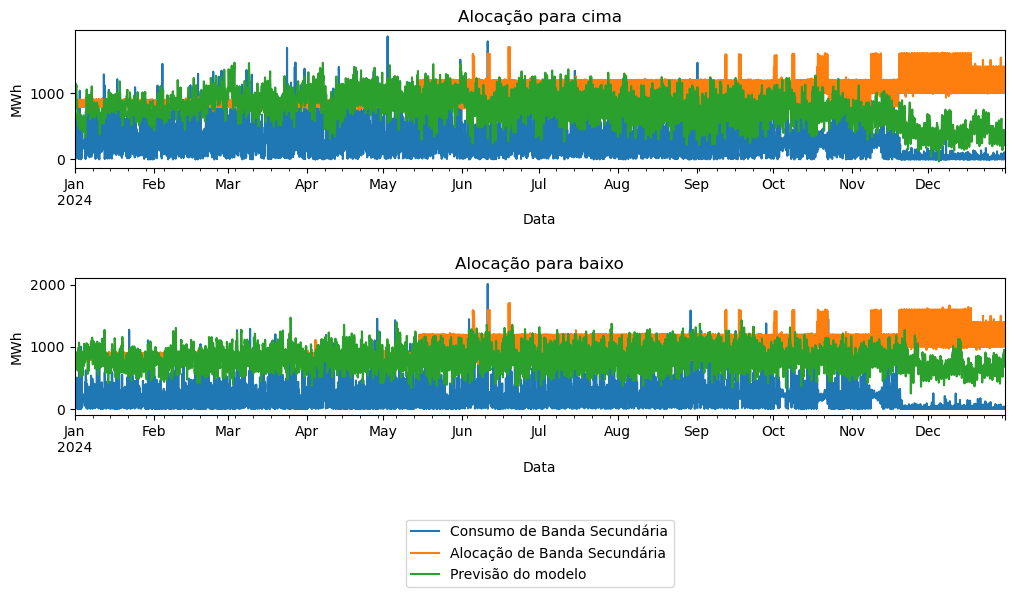
\includegraphics[width=\textwidth]{plots/alocacoes_finais.png}
    \caption{Série Temporal dos dados de validação}
    \label{fig:modeltimeseries}
\end{figure}

Esta figura apresenta os modelos finais durante toda a época de validação. nas secções seguintes vemos ao pormenor os resultados mais importantes de cada experiência.\par

\thispagestyle{plain}
\section{Estatísticos \label{se:resstats}}
Como ponto inicial de resultados os modelos estatísticos apresentam melhorias em relação à alocação em demasia, mas perdas significativas em relação a alocação em falta.\par

\begin{table}[H]
    \caption{Resultados métricas Modelos Estatísticos}    
    \resizebox{\linewidth}{!}{\begin{tabular}{llrrrrrrrrr}
\toprule
 &  & RMSE & SAE & AllocF & AllocD & GPD & GPD F & GPD D & GPD norm & GPD Positivo \\
 & Arquitetura &  &  &  &  &  &  &  &  &  \\
\midrule
\multirow[t]{3}{*}{Alocação a Subir} & ar & 169.21 & 4352584.52 & 2136545.80 & 2216038.73 & 74.92 & -1299.37 & 87.12 & -606.13 & 0.00 \\
 & arma & 181.33 & 4783841.06 & 2187173.52 & 2596667.54 & 72.44 & -1332.53 & 84.91 & -623.81 & 0.00 \\
 & ma & 183.10 & 4940770.16 & 2066116.05 & 2874654.11 & 71.54 & -1253.24 & 83.29 & -584.97 & 0.00 \\
\cline{1-11}
\multirow[t]{3}{*}{Alocação a Descer} & ar & 198.75 & 5265558.19 & 2624914.00 & 2640644.18 & 59.44 & -447.78 & 78.88 & -184.45 & 0.00 \\
 & arma & 218.76 & 5847476.54 & 2876213.76 & 2971262.78 & 54.96 & -500.22 & 76.23 & -211.99 & 0.00 \\
 & ma & 217.53 & 5869239.18 & 2871295.12 & 2997944.06 & 54.79 & -499.20 & 76.02 & -211.59 & 0.00 \\
\cline{1-11}
\bottomrule
\end{tabular}
}
    \label{tab:statsmetrics}
    \end{table}

Estes valores, a nível operacional, podem ser equiparáveis a alocar pouca ou nenhuma energia. Não correndo riscos de alocar em demasia. O que melhora bastante o desempenho em relação ao benchmark a nível de valor de energia absoluta desperdiçada mas derrota o propósito das reservas de energia.\par

\begin{figure}[H]
    \centering
    \includegraphics[width=\textwidth]{plots/alocacoes_temporais_upward_prediction_gpd_stats.png}
    \caption{Janelas temporais de modelos estatísticos energia a subir}
    \label{fig:statstimewindowsup}
\end{figure}


\begin{figure}[H]
    \centering
    \includegraphics[width=\textwidth]{plots/alocacoes_temporais_downward_prediction_gpd_stats.png}
    \caption{Janelas temporais de modelos estatísticos energia a descer}
    \label{fig:statstimewindowsdown}
\end{figure}

Estas figuras mostram que os modelos conseguem até acompanhar o real, podendo até ser um caminho a seguir com algum trabalho específico, mas perdem por manterem-se quase sempre abaixo do necessário, não dando assim a operacionalidade necessária à rede.\par
As médias horárias são:\\
\begin{table}[H]
    \resizebox{\linewidth}{!}{\begin{tabular}{llllll}
\toprule
 &  & média & desvio padrão & min & max \\
\midrule
\multirow[t]{2}{*}{Alocação a Descer (MW)} & benchmark & 542.59 & 126.09 & 363.00 & 946.00 \\
 & modelo & 200.14 & 103.62 & 0.00 & 915.37 \\
\cline{1-6}
\multirow[t]{2}{*}{Alocação a Subir (MW)} & benchmark & 623.68 & 152.39 & 419.00 & 958.00 \\
 & modelo & 160.49 & 77.05 & 0.00 & 765.82 \\
\cline{1-6}
\multirow[t]{2}{*}{Capacidade Horária (MW)} & benchmark & 1166.27 & 250.19 & 816.00 & 1891.00 \\
 & modelo & 360.63 & 109.25 & 45.53 & 1039.76 \\
\cline{1-6}
\multirow[t]{2}{*}{Energia a Descer Extraordinária (MWh)} & benchmark & 169.93 & 153.95 & 0.10 & 1226.40 \\
 & modelo & 192.13 & 168.57 & 0.00 & 1481.53 \\
\cline{1-6}
\multirow[t]{2}{*}{Energia a Subir Extraordinária (MWh)} & benchmark & 139.31 & 136.45 & 0.40 & 922.80 \\
 & modelo & 180.43 & 164.43 & 0.01 & 1508.90 \\
\cline{1-6}
\bottomrule
\end{tabular}
}
    \caption{Resultados Modelos Estatísticos}
    \label{tab:statsres}
    \end{table}



\begin{table}[H]
    \resizebox{\linewidth}{!}{\begin{tabular}{rrrrr}
\toprule
Alocação a Descer & Alocação a Subir & Capacidade Horária & Energia a Descer Extraordinária & Energia a Subir Extraordinária \\
\midrule
-63.11 & -74.28 & -69.08 & 13.06 & 29.65 \\
\bottomrule
\end{tabular}
}
    \caption{$\Delta$\% das médias dos Modelos Estatísticos}    
    \label{tab:statsres_deltas}
    \end{table}

As médias de alocação são bem mais baixas que o benchmark, mas este modelos têm bastante falta de energia alocada em ambas, logo não respondem à premissa base de ter menos energia em falta e em demasia, inclusivo têm um aumento de necessidade de uso de reserva terciária.\par


\thispagestyle{plain}
\subsection{Redes Neuronais \label{se:resml}}

Os vários métodos percorreram muitos tipos de modelos diferentes. Na tabela seguinte apresentamos apenas os melhores resultados baseados em GPD Positivo\par


\begin{table}[H]
    \caption{Resultados métricas Modelos Neuronais}    
    \resizebox{\linewidth}{!}{\begin{tabular}{llrrrrrrrrr}
\toprule
 &  & RMSE & SAE & AllocF & AllocD & GPD & GPD F & GPD D & GPD norm & GPD Positivo \\
 & Arquitetura &  &  &  &  &  &  &  &  &  \\
\midrule
\multirow[t]{5}{*}{Alocação a Subir} & UNET200 & 317.86 & 9759154.87 & 151181.25 & 9607973.62 & 43.78 & 0.98 & 44.16 & 22.57 & 43.78 \\
 & VanillaCNN200 & 328.88 & 10208138.49 & 147549.10 & 10060589.40 & 41.19 & 3.36 & 41.53 & 22.44 & 41.19 \\
 & UNET & 349.91 & 11008787.25 & 146742.39 & 10862044.86 & 36.58 & 3.89 & 36.87 & 20.38 & 36.58 \\
 & VanillaCNN & 370.73 & 11804382.23 & 149719.91 & 11654662.32 & 31.99 & 1.94 & 32.26 & 17.10 & 31.99 \\
 & 2StackedCNN200 & 410.28 & 13223932.55 & 126341.23 & 13097591.32 & 23.82 & 17.25 & 23.87 & 20.56 & 23.82 \\
\cline{1-11}
\multirow[t]{5}{*}{Alocação a Descer} & UNET200 & 282.52 & 8243468.87 & 469060.52 & 7774408.35 & 36.50 & 2.11 & 37.82 & 19.97 & 36.50 \\
 & VanillaCNN200 & 289.59 & 8671975.58 & 476040.73 & 8195934.85 & 33.20 & 0.66 & 34.45 & 17.55 & 33.20 \\
 & UNET & 304.28 & 9172373.23 & 470149.87 & 8702223.36 & 29.34 & 1.89 & 30.40 & 16.14 & 29.34 \\
 & VanillaCNN & 313.42 & 9483287.93 & 475881.60 & 9007406.33 & 26.95 & 0.69 & 27.95 & 14.32 & 26.95 \\
 & VanillaFCNN200 & 344.05 & 10438899.42 & 476740.17 & 9962159.25 & 19.59 & 0.51 & 20.32 & 10.41 & 19.59 \\
\cline{1-11}
\bottomrule
\end{tabular}
}
    \label{tab:mlresmetrics}
    \end{table}

O melhor modelo para alocação a Descer apresenta um ganho de desempenho em relação ao \textit{benchmark} de 42\%, e o a Subir de 47\% na soma da janela temporal de validação.\par
Estes modelos têm ambas as alocações e os erros menores que o \textit{benchmark}. Considerando que os dados que permitem quantificar a mais valia económica de reduzir a alocação de reserva secundária em falta devido não são dados públicos, o objetivo passa por manter esta alocações com valores mais baixos que o \textit{benchmark} (GPDF positivo mas próximo de 0) e minimizar a alocação em excesso, maximizando o GPDD, ou juntando as condições maximizando o GPD Positivo. Desta forma a primeira arquitetura de cada tabela é aquela que apresenta melhores resultados quantificáveis quer do ponto de vista operacional como económico.\par
Escolhendo o modelo com melhores resultados em GPD Positivo podemos ver algumas janelas temporais.\par


\begin{figure}[H]
    \centering
    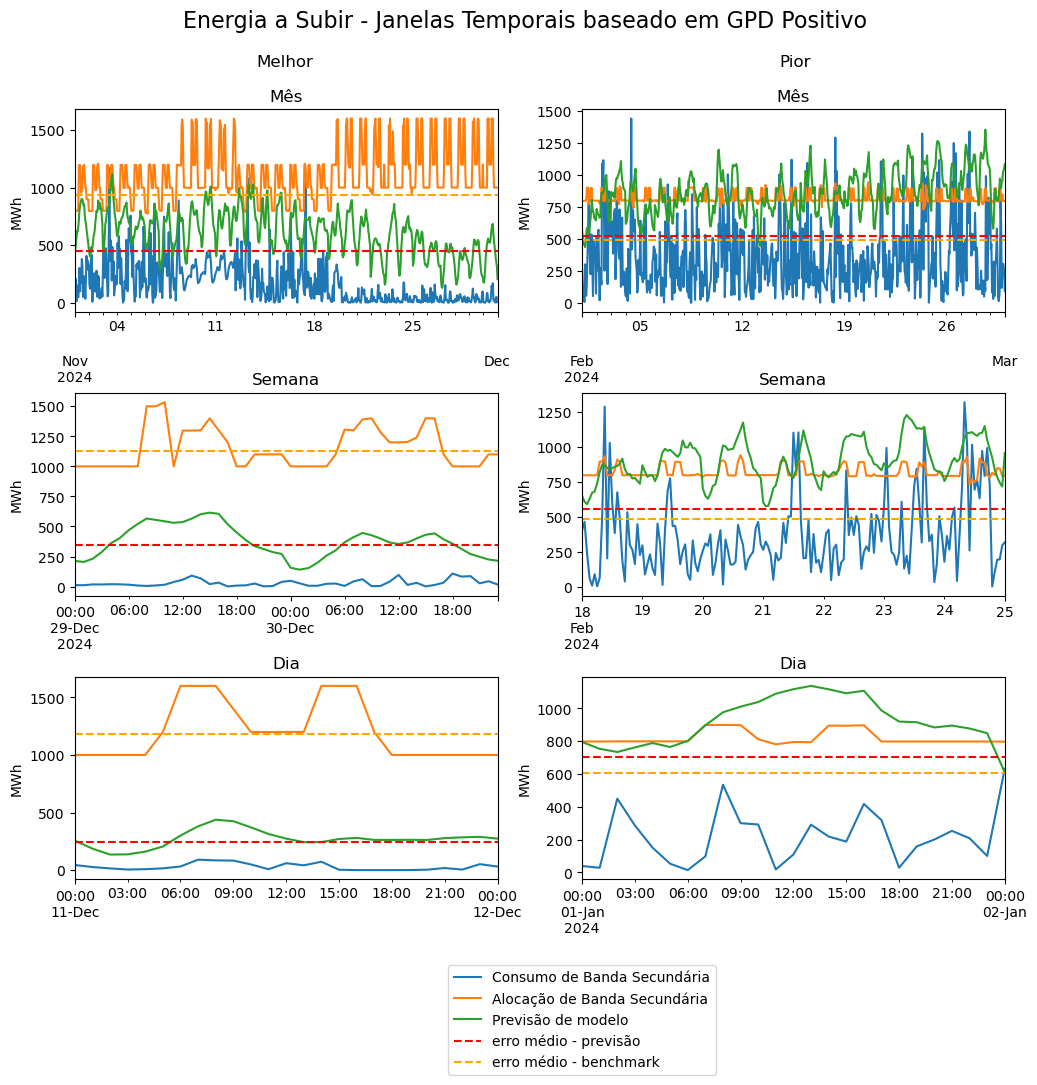
\includegraphics[width=\textwidth]{plots/alocacoes_temporais_upward_prediction_gpd_p.png}
    \caption{Janelas temporais energia a subir}
    \label{fig:mltimewindowsup}
\end{figure}


\begin{figure}[H]
    \centering
    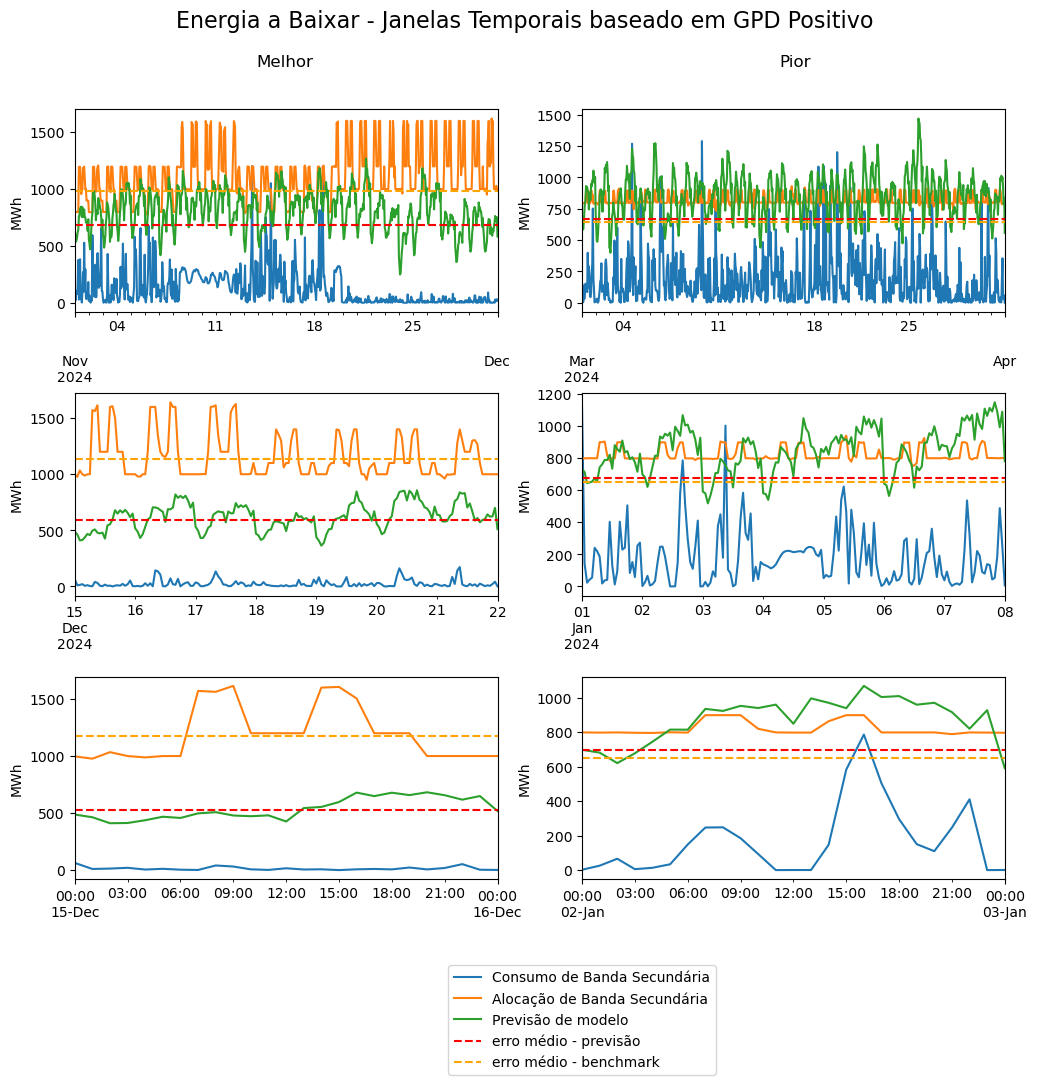
\includegraphics[width=\textwidth]{plots/alocacoes_temporais_downward_prediction_gpd_p.png}
    \caption{Janelas temporais energia a descer}
    \label{fig:mltimewindowsdown}
\end{figure}

É visualmente notável que o modelo mantém uma previsão mais perto da energia usada do que o \textit{benchmark}. Mesmo nas piores janelas temporais, o erro de previsão acumulado é claramente menor que o do método actual.\par
Atente-se no facto de as previsões seguirem bastante mais fielmente as curvas e picos apresentados nos valores de alocação reais, especialmente nas janelas de mês onde temos mais amostras. É possível perceber que o modelo quase sempre acompanha picos da energia usada voltado a baixar quando estes também baixam, destacando-se assim do actual método que mantém uma linha de base bastante mais elevada (desperdiçando mais recursos) e com flutuações que não descrevem tão bem a realidade.\par
Esta flexibilidade no modelo de redes neuronais permite ao operador ter um sinal muito mais flexível diminuindo, deste modo, a alocação desperdiçada.\par

\begin{figure}[H]
    \centering
    \includegraphics[width=\textwidth]{plots/alocation_sum_over_time.png}
    \caption{Soma de Banda Secundária}
    \label{fig:mltimewindowssum}
\end{figure}

Os gráficos anteriores vêm realçar esta mesma ideia. Analisando a energia cumulativa dentro janelas em destaque percebemos que o método proposto mantém quase sempre uma melhoria relativamente ao método utilizado. Esta melhoria é igualmente visível mesmo quando passamos a janelas diárias e semanais, embora haja um aumento considerável das vezes em que o método proposto não é melhor que o actual. E mais importante, o desenho das flutuações é bastante mais fiel ao real.\par


\begin{table}[H]
    \centering
    \caption{Resultados Modelos}    
    \resizebox{0.8\linewidth}{!}{\begin{table}[H] 
    \caption{Model Results and (allocated) values wthin 2024.\label{model_vs_bench}}
    \begin{adjustwidth}{-\extralength}{0cm}
    \newcolumntype{C}{>{\centering\arraybackslash}X}
    \begin{tabularx}{\fulllength}{CCCCCC}
    \toprule
    & & \textbf{mean}	& \textbf{std}	& \textbf{min} & \textbf{max}\\


    \midrule
            \multirow[m]{2}{*}{Down Allocation (MW)}	        & & (921.84) & (191.03) & (720.00) & (1708.00) \\
                                                                & & 836.85 & 182.04 & 247.82 & 1469.62 \\
            \multirow[m]{2}{*}{Up Allocation (MW)}	            & & (921.49) & (191.72) & (719.00) & (1694.00) \\
                                                                & & 778.42 & 228.85 & -29.47 & 1458.01 \\
            \multirow[m]{2}{*}{Hourly Capacity (MW)}	        & & (1843.32) & (382.35) & (1439.00) & (3399.00) \\
                                                                & & 1615.27 & 346.50 & 393.85 & 2594.85 \\
            \multirow[m]{2}{*}{Extraordinary Down Energy (MWh)}	& & (168.74) & (175.69) & (0.90) & (1214.00) \\
                                                                & & 149.66 & 179.96 & 2.66 & 1358.81 \\   
            \multirow[m]{2}{*}{Extraordinary Up Energy (MWh)}	& & (179.39) & (163.94) & (1.00) & (1054.80) \\
                                                                & & 141.85 & 153.57 & 1.83 & 1420.22 \\
    \bottomrule
    \end{tabularx}
    \end{adjustwidth}
\end{table}
}
    \label{tab:mlres}
    \end{table}



\begin{table}[H]
    \caption{$\Delta$\% das médias dos Modelos}    
    \resizebox{\linewidth}{!}{\begin{table}[H] 
    \caption{Mean $\Delta$\% between model and benchmark\label{model_vs_bench_perc}}
    \newcolumntype{C}{>{\centering\arraybackslash}X}
    \begin{tabularx}{\textwidth}{CC}
    \toprule
    & \textbf{$\Delta$\%} \\
    

    \midrule
            Down Allocation (MW)	        & -28.62 \\
            Up Allocation (MW)              & -37.26 \\
            Hourly Capacity (MW)	        & -33.24 \\
            Extraordinary Down Energy (MWh)	& -51.62 \\
            Extraordinary Up Energy (MWh)	& -59.47 \\
    \bottomrule
    \end{tabularx}
    % \noindent{\footnotesize{\textsuperscript{1} Tables may have a footer.}}
\end{table}


}
    \label{tab:mlres_deltas}
    \end{table}

O método proposto apresenta uma melhoria total, durante o período de validação, de \textasciitilde47\% na alocação a subir e \textasciitilde42\% na alocação a descer face ao método usado no mercado. As melhorias médias são de \textasciitilde37\% e \textasciitilde29\% respectivamente, o que também é uma melhoria face ao estado da arte \cite{Algarvio2024} com 13\% e 8\%.\par
O método proposto liberta em média \textasciitilde33\% dos recursos horários, e baixando a necessidade de activar a reserva terciária em \textasciitilde52\% e \textasciitilde59\%.\par

As correlações entre o modelo e a realidade são também mais elevadas que entre \hyperref[fig:featurecorrelation]{modelo e \textit{benchmark}}.


\begin{figure}[H]
    \centering
    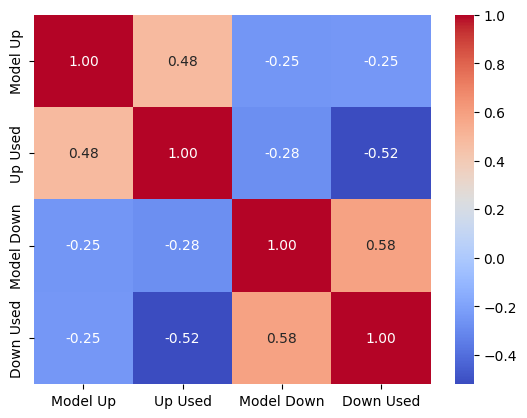
\includegraphics[width=0.8\textwidth]{plots/heatmap_correlation_pred.png}
    \caption{Correlação entre previsão e real}
    \label{fig:predcorrelation}
  \end{figure}

Este mapa de correlações é quase o oposto do apresentado pelo \hyperref[fig:benchmarkcorr]{\textit{benchmark}}.\par
Aqui as correlações maiores são, como seria de esperar, entre a energia usada e a sua alocaçao. Com 48\% na energia a subir e 58\% a descer. E as energias alocadas têm uma correlaçao baixa.\par 
